\documentclass[a4paper,12pt]{article}
	\usepackage{graphicx}
	\usepackage[utf8]{inputenc}
	\usepackage[T1]{fontenc}
	\usepackage{listings}
	\usepackage{color}
	\usepackage{amsmath}

	\definecolor{dkgreen}{rgb}{0,0.6,0}
	\definecolor{gray}{rgb}{0.5,0.5,0.5}
	\definecolor{mauve}{rgb}{0.58,0,0.82}

	\lstset{frame=tb,
	  language=Python,
	  aboveskip=3mm,
	  belowskip=3mm,
	  showstringspaces=false,
	  columns=flexible,
	  basicstyle={\small\ttfamily},
	  numbers=none,
	  numberstyle=\tiny\color{gray},
	  keywordstyle=\color{blue},
	  commentstyle=\color{dkgreen},
	  stringstyle=\color{mauve},
	  breaklines=true,
	  breakatwhitespace=true
	  tabsize=3
	}
	\title{ Mecânica Clássica I}
	\author{\small André Del Bianco Giuffrida\\ \small IFSC - USP\\ \small andre.giuffrida@usp.br}
	\date{}
\begin{document}
\maketitle
	Oscilador Harmonico amortecido!
	
	Como:
	\[ F = -kx -b\dot{x}\]
	Obtemos a Equação Diferencial:
	\[ \ddot{x} + \frac{b}{m}\dot{x} + \frac{k}{m}x = 0\]
	Como a solução é clássica vamos testar o Ansatz :
	\[x(t) = e^{pt} \]
	Isso pois:
	\[\dot{x}(t) = pe^{pt} \]
	\[\ddot{x}(t) = p^2e^{pt} \]
	Substituindo na equação diferencial obtemos o seguinte:
	\[ \Bigg[ p^2 + p\frac{b}{m} + \frac{k}{m} \Bigg]e^{pt}= 0 \]
	Para satisfazer a equação teremos que resolver a equação de segundo grau entre colchetes para $p$.
	Sendo assim:
	\[ p = \frac{ -\frac{b}{m} \pm \sqrt{\Big(\frac{b}{m}\Big)^{2} - 4\frac{k}{m} } }{2}\]
	Com o intuito de simplificar faremos: 
	\[\frac{b}{2m} = \gamma \quad \text{e} \quad \frac{k}{m}=\omega^2\]
	temos, por fim.
	\[ p = \frac{ -\gamma}{2} \pm \sqrt{\gamma^2 - \omega^2}\]
	O que faz, com que $x(t)$ tenha duas soluções.
	e por isso, $x(t)$ é uma combinação linear ($x = \alpha x_1 + \beta x_2 $) das duas.
	ou seja:
	\[ x(t) =  \alpha e^{\frac{ -\gamma t}{2} + \sqrt{\gamma^2 - \omega^2}t} + \beta e^{\frac{ -\gamma}{2} - \sqrt{\gamma^2 - \omega^2} t}\]
	\[ x(t) =  e^{\frac{ -\gamma t}{2}} \Big[\alpha e^{\sqrt{\gamma^2 - \omega^2}t} + \beta e^{- \sqrt{\gamma^2 - \omega^2}t} \Big]\]
	
	Agora podemos analisar os diversos casos para $\gamma$ e $\omega$.
	\begin{itemize}
	\item Para  $\gamma < \omega$.
	
		Note que a raiz $\sqrt{\gamma^2 - \omega^2}$ torna-se complexa, podendo ser reescrita como:
		\[ i\sqrt{\omega^2 - \gamma^2} \]
		O que faz de $x(t)$ possuir uma componente complexa.
		\[ x(t) = e^{\frac{ -\gamma t }{2}} \Big[\alpha e^{i\sqrt{\omega^2 - \gamma^2 }t} + \beta e^{-i\sqrt{\omega^2 - \gamma^2 }t} \Big] \]
		Lembrando da Formula de Euler podemos substituir as exponenciais complexas por senos e cossenos.
		\[ e^{i\theta} = cos(\theta) + isin(\theta)\]
		e assim podemos fazer a substituição
		\[ \sqrt{\omega^2 - \gamma^2 } = \Omega \]
		Para ficar-mos com:
		\[  x(t) = e^{\frac{ -\gamma t}{2}}\Big[ \alpha[ cos(\Omega t)+isin(\Omega t) ] + \beta[sin(\Omega t ) +icos(\Omega t)] \Big]\]
		Como não estamos interessados na parte imaginária ficamos com:
		\[  x(t) = e^{\frac{ -\gamma t}{2}}\Big[ \alpha cos(\Omega t)+\beta sin(\Omega t) \Big]\]
		Que pode ser reescrito como:
		\[  x(t) = e^{\frac{ -\gamma t}{2}} A cos(\Omega t + \theta_0)\]
	
	\begin{figure}[h]
		\centering
		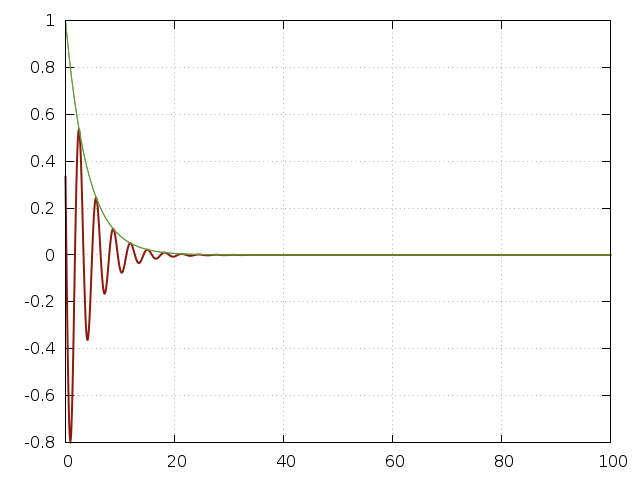
\includegraphics[scale=0.6]{7o0.png}
		\caption{Subamortecimento - em verde o decamimento: $e^{-\frac{\gamma}{2}t}$}
	\end{figure}
	
	\item Para  $\gamma > \omega$.
	
		Nesse caso não temos o termo complexo ou seja a raiz $\sqrt{\gamma^2 - \omega^2}$ é real fazendo com que
		\[ x(t) =  e^{\frac{ -\gamma t}{2}} \Big[\alpha e^{\sqrt{\gamma^2 - \omega^2}t} + \beta e^{- \sqrt{\gamma^2 - \omega^2}t} \Big]\]
		onde as constantes $\alpha$ e $\beta$  dependem das condições iniciais:
		\[ x(0) = \alpha + \beta = x_0 \]
		\[ \dot{x}(0) = \frac{ -\gamma}{2} [ \alpha + \beta] + [\alpha - \beta ]\sqrt{\gamma^2 - \omega^2} = 0\]
		\[\frac{ \gamma}{2} x_0 = [2\alpha - x_0]\sqrt{\gamma^2 - \omega^2}\]
		\[\alpha = \frac{ \gamma x_0}{4 \sqrt{\gamma^2 - \omega^2}}  + \frac{x_0}{2}\]
			
	\begin{figure}[h]
		\centering
		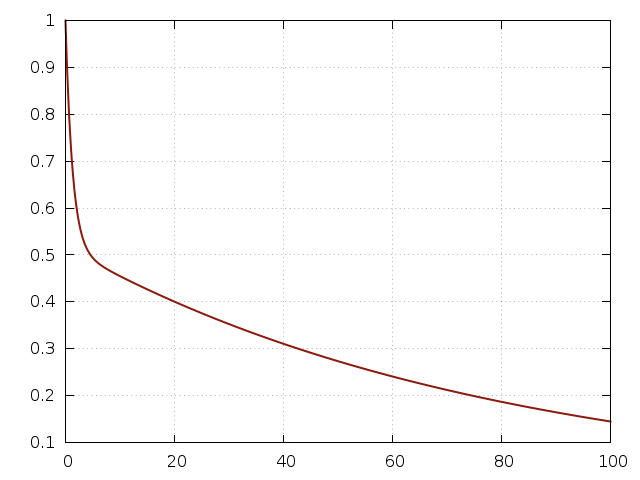
\includegraphics[scale=0.6]{7o1.png}
		\caption{Amortecimento}
	\end{figure}
	
	\item Para  $\gamma = \omega$.
	Aqui vamos voltar na equação diferencial, e substituir nela.
	
	\[ \ddot{x} + \frac{b}{m}\dot{x} + \frac{k}{m}x = 0\]
	\[ \frac{b}{m}  = 2\gamma \quad \text{e} \quad \frac{k}{m} = \omega^2\]
	o que nos dá:
	\[ \ddot{x} + 2\gamma\dot{x} + \gamma^2x = 0\]
	agora temos algo diferente na Equação Diferencial e isso leva em um novo ansatz:
	\[x(t) = f(t)e^{st} \]
	pois:
	\[\dot{x}(t) = \dot{f}(t)e^{st} + f(t)se^{st}  \]
	\[\ddot{x}(t) = \ddot{f}(t)e^{st} + 2\dot{f}(t)se^{st} + f(t)s^2e^{st}  \]
	substituindo na Equação inicial obtemos:
	\[ \ddot{f}(t)e^{st} + 2\dot{f}(t)se^{st} + f(t)s^2e^{st} + 2\gamma \Big[ \dot{f}(t)e^{st} + f(t)se^{st} \Big] + \gamma^2 \Big[f(t)e^{st} \Big] = 0\]
	\[ \ddot{f}(t) + 2\dot{f}(t)s + f(t)s^2+ 2\gamma \Big[ \dot{f}(t) + f(t)s\Big] + \gamma^2 \Big[f(t) \Big] = 0\]
	\[ \ddot{f}(t) + \dot{f}(t) \Big[2s+ 2\gamma\Big] + f(t) \Big[s^2+2\gamma s+\gamma^2  \Big] = 0\]
	Note o quadrado perfeito.
	\[ \ddot{f}(t) + 2\Big(s+ \gamma\Big)\dot{f}(t)  + \Big(s + \gamma\Big)^2 f(t) = 0\]	
	sendo $s = -\gamma$
	\[ \ddot{f}(t) = 0\]
	o que leva a 
	\[ f(t) = f_0 + f_1 t\]
	\[ x(t) = (f_0 + f_1 t )e^{-\gamma t}\]
	vemos que utilizando as condições iniciais, as constantes $f_0 $ e $f_1$ podem ser encontradas como segue:
	\[x(0) = f_0 = x_0\]
	\[\dot{x}(t) = 0 = f_1 - \gamma f_0 \to  f_1 = \gamma x_0 \]
	Podemos escrever.
	\[ x(t) = (x_0 + \gamma x_0 t)e^{-\gamma t}\]
	
	\begin{figure}[h]
		\centering
		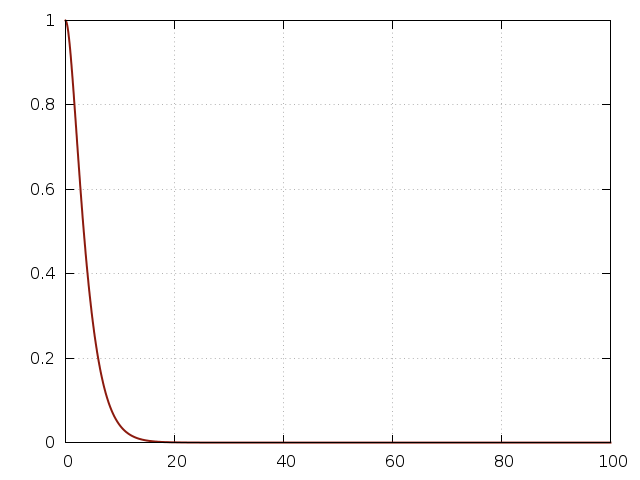
\includegraphics[scale=0.6]{7o2.png}
		\caption{Amortecimento Crítico}
	\end{figure}
	
	\end{itemize}
	
	\end{document}
	
